% !TEX TS-program = XeLaTeX
%!TEX encoding = UTF-8 Unicode
%-------------------------------------------------------
% Author: Christian Häusler based on the work from Thomas Bruderer
% Email: christian.haeusler@piratenpartei.ch
%-------------------------------------------------------

% -------------------------------------------
% Use the following options to customize
% -------------------------------------------
% aspectratio
%	1610	≙	16:10
%	169	≙	16:9
%	149	≙	14:9
%	54	≙	5:4
%	43	≙	4.3
%	32	≙	3:2
%
% [bigger, smaller] use either to change the
% size or non of them for the default
\documentclass[aspectratio=1610, compress, bigger]{beamer}
% -------------------------------------------
% Use the following three lines instead of the above 
% to create a handout
% -------------------------------------------
%\documentclass{scrartcl}
%\usepackage{ppsdocument}
%\usepackage[noxcolor, hyperref]{beamerarticle}

% -------------------------------------------
% Load the pps beamer theme
% Possible options are:
%	miniframes (use the outer theme miniframes)
%	structured (use the outer theme sidebar)
%		right (display the sidebar on the right side)
%		left (display the sidebar on the left side: default)
%		width=<dimension> (width of the sidebar)
%		heifht=<dimension> (height of the frame title)
% -------------------------------------------
\usetheme{pps}
 
% -------------------------------------------
% Uncomment one of the following lines for a section
% specific document
% -------------------------------------------
%\usepackage{ppsag} % Aargau
%\usepackage{ppsbb} % Beide Basel
%\usepackage{ppsbe} % Bern / Berne
%\usepackage{ppsfr} % Freiburg / Fribourg
%\usepackage{ppsos} % Ostschweiz: St. Gallen und beide Appenzell
%\usepackage{ppsvd} % Vaudoise
%\usepackage{ppszh} % Zürich
%\usepackage{ppszs} % Zentralschweiz

% Do not show the navigation symbols
\beamertemplatenavigationsymbolsempty

% -------------------------------------------
% Change from here
% -------------------------------------------
\title[Pi-Vote]{The Pi-Vote eVoting System}
%\subtitle<presentation>[Short subtitle]{Subtitle in full length}
\subtitle{How the Pirate Party Switzerland uses ADDER}
\author[D. Simonet, S. Thöni]{Denis Simonet, Stefan Thöni}
\date[\today]{\today}
\subject{The Pi-Vote eVoting System: How the Pirate Party Switzerland uses ADDER}
\keywords{Pi-Vote, eVoting, ADDER}

\begin{document}
% -------------------------------------------
% Set the language will also change the logo
% Possible options are:
% 	english
% 	french
% 	italian
% 	ngerman
% -------------------------------------------
\selectlanguage{english}

% -------------------------------------------
% Change background color
% ------------------------------------------
% The following commands can be used to
% change the background color for the slides
%
% \backgrounddefault
% \backgroundorange
% \backgroundviolet
% \backgroundgrey
% -------------------------------------------

\frame[plain]{\maketitle}

%\section<presentation>{This section exists only in the presentation modes}
%\section<article>{This section exists only in the article mode}
%\section[Summary]{Summary of Main Results}
%\hyperlink{somewhere}{\beamerbutton{Go somewhere}}

% Toc only shown in the handout
\frame<article>[plain]{\tableofcontents\newpage}

\part[Part 1]{Why does the Pirate Party Switzerland use eVoting?}

\frame[plain]{\partpage}

\section{Intro} 
\begin{frame}\frametitle{About Pi-Vote} 
\begin{center}
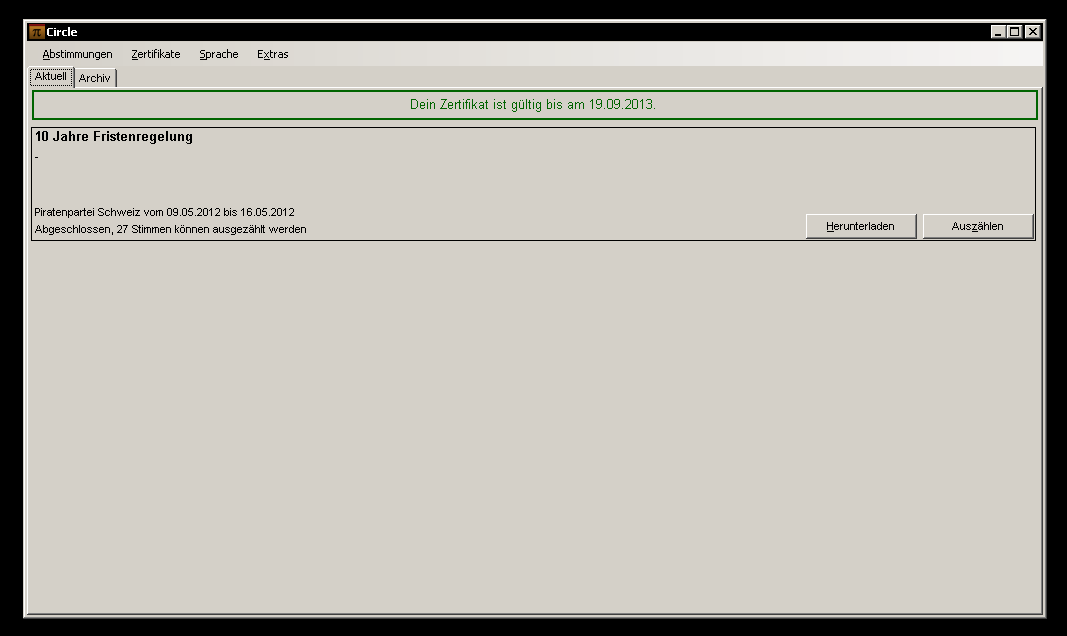
\includegraphics[width=12cm]{pivote.png}
\end{center}
\end{frame}

\part[Part 2]{How Pi-Vote works and what Problems remain}

\frame[plain]{\partpage}

\section{Assumptions}
\begin{frame}\frametitle{Assumptions}

\begin{block}{We assume...}
\begin{itemize}
\item Decisional Diffie-Hellman assumption is true;
\item Integer factorization is hard;
\item SHA-2 is sufficiently close to a random oracle;
\item Random number generators in PCs/OS are good.
\end{itemize}
\end{block}

\end{frame}

\section{Secrecy}
\begin{frame}\frametitle{Secrecy}

\begin{block}{How is secrecy achieved?}
\begin{itemize}
\item Homomorphic encryption of ballots
\item 4 out of 5 sharing of the secret
\end{itemize}
\end{block}

\pause

\begin{alertblock}{Potential problems}
\begin{itemize}
\item Possibility of decryption exists and could be forced e.g. by law
\item Parts of secret may be lost or given away later
\end{itemize}
\end{alertblock}

\pause

\begin{alertblock}{Real problems}
\begin{itemize}
\item Authorities can be unreliable!
\end{itemize}
\end{alertblock}

\end{frame}

\section{Correctness}
\begin{frame}\frametitle{Correctness}

\begin{block}{How is the correctness of ballots ensured?}
\begin{itemize}
\item Zero knowledge proofs with Fiat-Shamir heuristic
\end{itemize}
\end{block}

\pause

\begin{alertblock}{Real problems}
\begin{itemize}
\item Proofs take many CPU cycles to verify
\end{itemize}
\end{alertblock}

\end{frame}

\section{Authorization}
\begin{frame}\frametitle{Authorization}

\begin{block}{How is voting authorized?}
\begin{itemize}
\item RSA signatures
\item Certificates
\end{itemize}
\end{block}

\pause

\begin{alertblock}{Potential problems}
\begin{itemize}
\item Compromised CA
\item Only achieves pseudonymity
\end{itemize}
\end{alertblock}

\end{frame}

\section{Authentication}
\begin{frame}\frametitle{Authentication}

\begin{block}{How are members authenticated?}
\begin{itemize}
\item Paper form 
\item 3 signatures from elected notaries
\end{itemize}
\end{block}

\pause

\begin{alertblock}{Potential problems}
\begin{itemize}
\item Forged signatures
\item Bribery and threat
\end{itemize}
\end{alertblock}

\pause

\begin{alertblock}{Real problems}
\begin{itemize}
\item Not easy enough to use
\end{itemize}
\end{alertblock}

\end{frame}

\section{Tallying}
\begin{frame}\frametitle{Tallying}

\begin{block}{How to guarantee re-tallying at any time?}
\begin{itemize}
\item Votes and partial decryptions are published and can be downloaded any time
\end{itemize}
\end{block}

\pause

\begin{alertblock}{Potential problems}
\begin{itemize}
\item Breaking software changes
\end{itemize}
\end{alertblock}

\end{frame}

\section{Receipt-freeness}
\begin{frame}\frametitle{Receipt-freeness}

\begin{block}{Is Pi-Vote receipt-free?}
\begin{itemize}
\item No
\item Not a requirement
\end{itemize}
\end{block}

\pause

\begin{block}{Possible solution}
\begin{itemize}
\item Ballot re-randomization
\end{itemize}
\end{block}

\end{frame}

\section{Manipulated software}
\begin{frame}\frametitle{Manipulated software}

\begin{block}{How to make sure the software is not manipulated?}
\begin{itemize}
\item Transparency, Open Source
\end{itemize}
\end{block}

\pause

\begin{alertblock}{Not good enough...}
\begin{itemize}
\item No one ever publicly checked the software security!
\item Most users simply download from our page
\end{itemize}
\end{alertblock}

\end{frame}

\section{Denial of service}
\begin{frame}\frametitle{Denial of service}

\begin{block}{Internal attacker}
\begin{itemize}
\item Delete the database
\item Shut down the server
\end{itemize}
\end{block}

\pause

\begin{block}{External attacker}
\begin{itemize}
\item Overload the server
\end{itemize}
\end{block}

\pause

\begin{alertblock}{Impossible to solve...}
\begin{itemize}
\item Hard to mitigate
\item Mostly a case for courts
\end{itemize}
\end{alertblock}

\end{frame}

\section{User acceptance}
\begin{frame}\frametitle{User acceptance}

\begin{block}{How do we achieve good user acceptance?}
\begin{itemize}
\item Open and transparent processes
\item Democratic voting on procedures
\end{itemize}
\end{block}

\pause

\begin{alertblock}{Real problems}
\begin{itemize}
\item Users don't understand what's going on but most don't care either
\item Multi-platform support and installation are trouble magnets
\item Documentation is insufficient
\item User interface is never satisfactory
\end{itemize}
\end{alertblock}

\end{frame}

\section{Future plans}
\begin{frame}\frametitle{Future plans}

\begin{block}{Process changes}
\begin{itemize}
\item Accept identification by Swiss Post and Communal Administration
\item Accept SuisseID
\end{itemize}
\end{block}

\pause

\begin{block}{Technical changes}
\begin{itemize}
\item Additional Java client
\item Android client
\item Hardware certificates
\end{itemize}
\end{block}

\end{frame}

\end{document}